\section{Monitoring Architecture Model}
\label{sec:arch}

% Run-time monitoring overview
\begin{figure}
  \begin{center}
    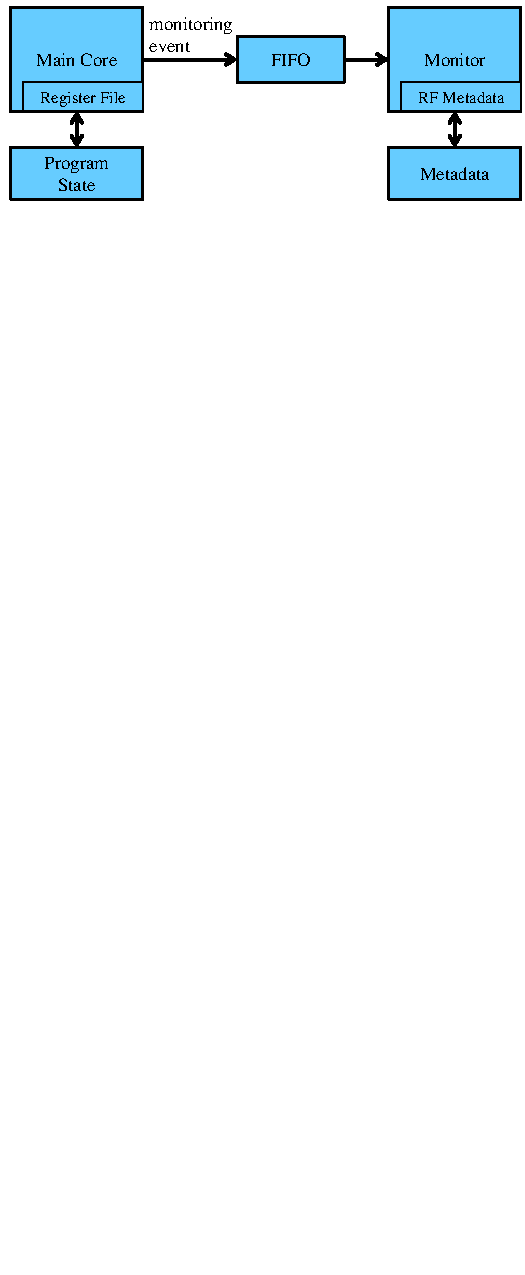
\includegraphics[width=\columnwidth]{figs/monitoring_architecture.pdf}
    \vspace{-0.2in}
    \caption{Overview of run-time monitoring architecture.}
    \label{fig:arch.overview} 
    \vspace{-0.2in}
  \end{center}
\end{figure}

Figure~\ref{fig:arch.overview} shows an overview of the run-time monitoring
model that is assumed in this paper. 
% The \emph{main task} is a computation task that performs the original function
% of the real-time system and is run on the \emph{main core}. 
The \emph{main program} is a computation task that performs the original
function of the system and is run on the \emph{main core}.
% The main task has a
% worst-case execution time (WCET) which can be upper-bounded using a variety
% of existing techniques \cite{wcetsurvey-tecs08}. This WCET is used for timing
% analysis in the design of the real-time system. As long as the execution
% time of the main task does not exceed this bound, then all timing guarantees
% from the analysis hold.
On certain events
during the main program, such as the execution of certain types of
instructions, the \emph{monitor} performs a series of \emph{monitoring
operations}. The monitor operates in parallel to the main core. These events
are referred to as
\emph{monitoring events}. Depending on the type of a monitoring event, different
monitoring operations are executed. Monitoring events are buffered
in a FIFO
structure to decouple the running of the main core and the monitor. If the FIFO
is full, then the main core is forced to stall on a monitoring event until a
FIFO entry becomes available. For programmable monitors, these stalls are a
major source of overhead because the monitor may take several cycles to process
a single event from the main core. We refer to these stalls and other
overheads,
such as contention for shared resources, as
\emph{monitoring overheads}. If the monitor detects an %inconsistent or
undesired behavior in the monitoring events, then an error is detected. 
% We do
% not focus here on the question on how to handle such an error. However, there are
% several options on how to handle an error such as raising an exception,
% notifying the user, or switching to a simpler, more trusted main task
% \cite{sha-simplex-sw01}.

There are many possible monitoring schemes that can be implemented on this
type of fine-grained parallel monitoring architecture such as
array bound checks \cite{devietti-hardbound-asplos08}, memory protection \cite{mmp02}, 
information flow tracking \cite{suh-dift-asplos04, greathouse-testudo-micro08}, 
soft error detection \cite{argus-micro07}, data-race detection \cite{cord-hpca06}, etc.
One example is an
uninitialized memory check (UMC) where 
monitoring is used to detect when software attempts to read from a memory location that
was not previously initialized. This can be done by forwarding each load and store
instruction from the main core to the monitor.
%the memory address
%of each store and load instruction on the main core to the monitor as
%well as whether the instruction was a store or load. 
For every memory location,
the monitor keeps one bit of metadata. On a store to a
memory location, the monitor marks the corresponding metadata bit to
indicate that the memory location has been initialized. On a load,
the monitor checks that the corresponding metadata bit has
been previously marked as initialized.

There are multiple options for implementing programmable parallel monitors. For example, the
Log-Based Architecture \cite{chen08-lba} uses processor cores in a multi-core
system as monitors. The FlexCore architecture \cite{deng-flexcore-micro10}
instead uses an FPGA-fabric to implement the monitor. The approach we describe
in this paper applies to any of these parallel monitors. However, for experiments,
we model an FPGA-based monitor similar to FlexCore. 
%Specifically, this
%architecture uses an on-chip FPGA fabric to
%allow high-performance and reconfigurable run-time monitoring. 
The on-chip FPGA fabric is
used to implement the ``Monitor'' block in Figure~\ref{fig:arch.overview}
while the FIFO from the main core and metadata cache are implemented as ASICs.
